% Sample file for AES paper
\documentclass{aes2e}
\usepackage[dvipsnames]{xcolor}
\usepackage{enumitem}
% Metadata Information
\jyear{2016}
\jmonth{May}
\jvol{1}
\jnum{1}


\begin{document}

% Page heads
\markboth{Castillo McQuiddy AND  Méndez Martínez}{Creating a File System Manager using Haskell}


% Title portion
\title{Creating a File System Manager using Haskell}

%Author Info.
\authorgroup{
\author{\quad\quad\quad\quad Cristian Castillo McQuiddy } \author{  \quad\quad Jairo Mendez Martínez }
\role{}
\newline(2014061245)\quad\quad\quad\quad\quad\quad\quad\quad\quad\quad (2014050475)
\affil{Instituto Tecnológico de Costa Rica}
}

%Abstract
\abstract{%
As part of this project  a file system is going to be written in haskell to emulate  functionality a file manager covering volumes, file systems and files management processes in Linux.
}


\maketitle

%Head 1
\section{INTRODUCTION}

On a UNIX system, everything is a file; if something is not a file, it is a process.A Linux system, just like UNIX, makes no difference between a file and a directory, since a directory is just a file containing names of other files. Programs, services, texts, images, and so forth, are all files. Input and output devices, and generally all devices, are considered to be files, according to the system, \cite{DEK1}. \newline

The Filesystem Hierarchy Standard (FHS) defines the main directories and their contents in Linux operating systems. For the most part, it is a formalization and extension of the traditional BSD filesystem hierarchy, as illustrated in  Figure 1. \cite{DEK2}.\newline.




%Figure
\begin{figure}[ht]
\centering
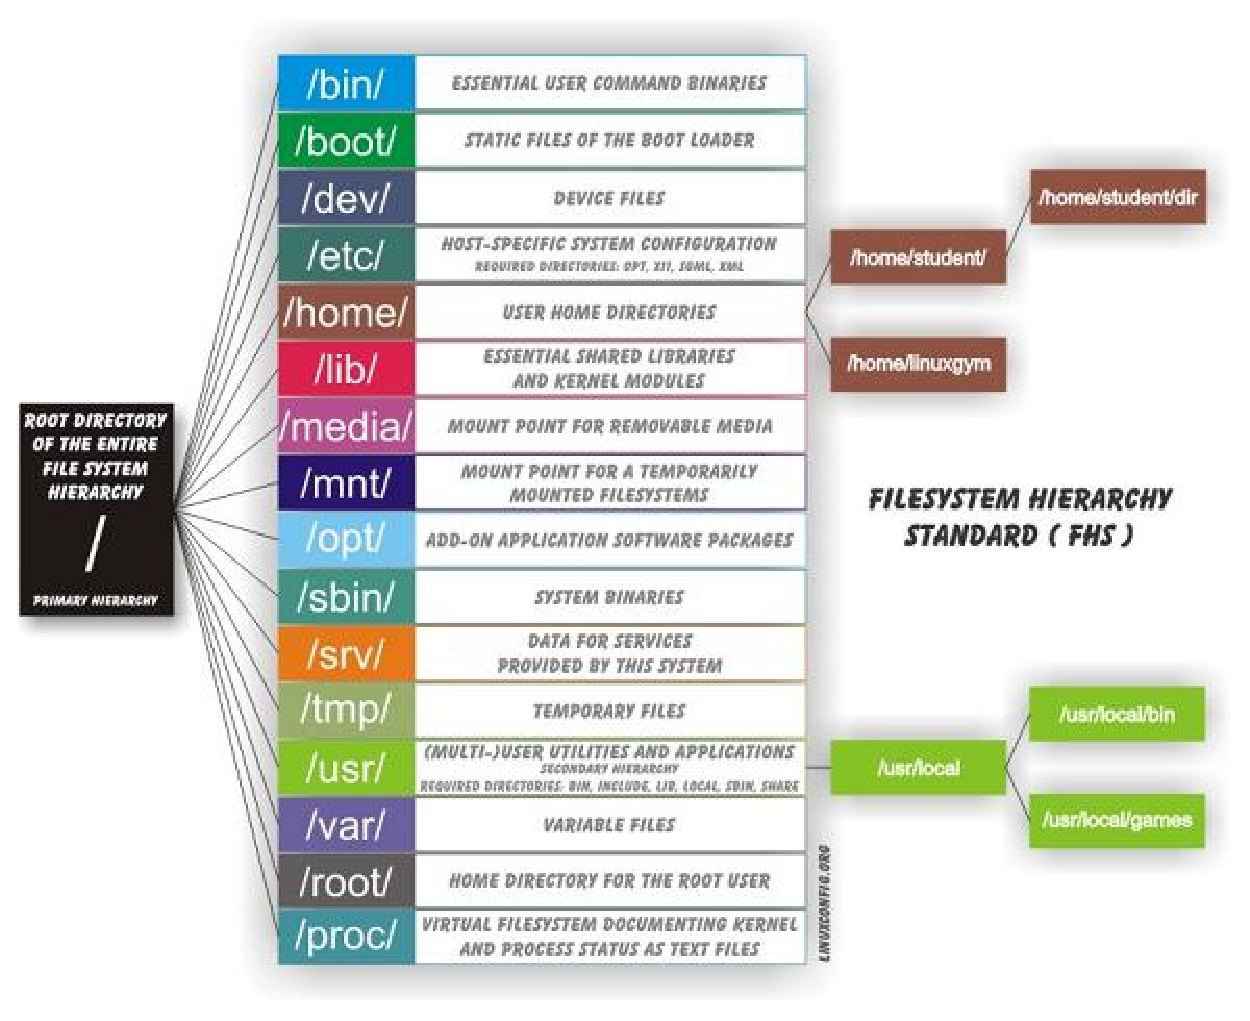
\includegraphics[width=20pc]{hN4lt.eps}
\caption{File System Hierarchy Standard (FHS).}
\end{figure}

Linux where made as multi-user systems t unlike Windows was created for a single user.\newline

A file system is used to control how data is stored and retrieved. Without a file system, information placed in a storage area would be one large body of data with no way to tell where one piece of information stops and the next begins. By separating the data into pieces and giving each piece a name, the information is easily isolated and identified. Taking its name from the way paper-based information systems are named, each group of data is called a "file". The structure and logic rules used to manage the groups of information and their names is called a \textbf{"file system"}.\cite{DEK2}\newline

Files have ownership composed by users and groups. Hence as part of this system, we will be able to manage basic \textbf{user and groups} to be able to setup the ownership in the file and directories that will be created in this system.\cite{DEK3}\newline

Linux uses more than one partition on the same disk.One of the goals of having different partitions is to achieve higher data security in case of disaster. By dividing the hard disk in partitions, data can be grouped and separated. When an accident occurs, only the data in the partition that got the hit will be damaged, while the data on the other partitions will most likely survive.\cite{DEK1} \newline

\textbf{Storage devices} will be created to emulate the equivalent to SAN LUNs, hard drives or any other storage device required to create a file system or a logical volume.Each storage device could initialize to be used by \textbf{LVM}\cite{DEK2} \newline

As illustrated in  Figure 2, logical volumes manager allow us to create a set of volumes where the file systems are going to be created over. The volume groups are formed by physical volumes (or storage devices) and volumes. A volume can be created using the total space allocated in the volume group and not to be limited by the size of a single storage device.\cite{DEK2} \newline

%Figure
\begin{figure}[ht]
\centering
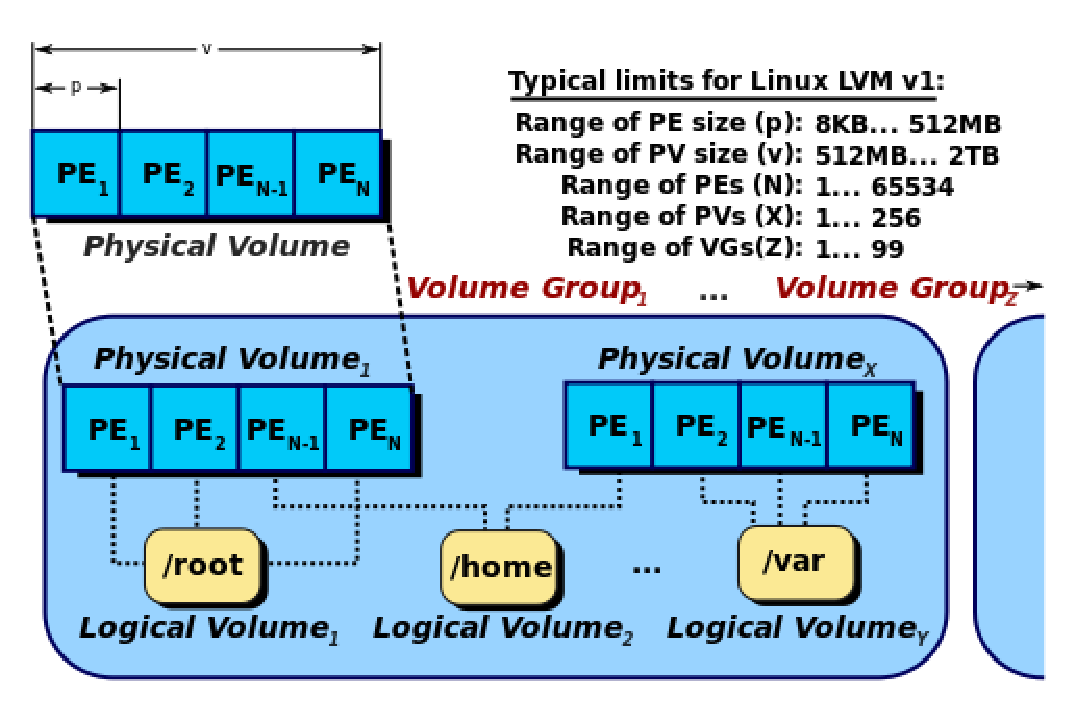
\includegraphics[width=20pc]{LVM.eps}
\caption{LVM (Logical Volume Manager).\cite{DEK4}}
\end{figure}

The file systems are going to be created over a single logical volume or over a specific storage device. \newline

The file system mount points are directories associated with an existent file system. Both the file systems and mount points need to be created in order to be able to associate them with each other.
To be able to use a file system to create files or directories inside of it, it needs to be mounted and mapped over an existent directory.\cite{DEK2} \newline

Haskell is a standardized, general-purpose purely functional programming language, with non-strict semantics and strong static typing. It was designed without any application niche in
mind. Although it takes a strong stand on how programs should be written, it does not favor one problem domain over others. While at its core, the language encourages a pure, lazy style of functional programming, this is the default, not the only option.\newline.

The program is going to interact with the user over the command line. The user will be triggering commands to be able to interact with the program. The program is go to display the
outputs of each of the operations requested by a user . The commands are going to impact the environment that is going to be managed by the file manager.\cite{DEK2} \newline

\section{Development environment}
The file system was implemented in Linux , and was developed using haskell language, which is an functional language, this one can be implemented in any haskell IDLE, for the development for this investigation SublimeText3 is the one that was used, this one can be downloaded in \cite{DEK5}.\newline\newline



\section{Libraries}
\begin{itemize}
\item{}\textcolor{Magenta}{import} \textcolor{blue} {Data.Tuple.Select} : Used for the structures of the file system\newline

\item{}\textcolor{Magenta}{import} \textcolor{blue} {Data.List.Split} : Used to split some symbols like spaces " ".\newline

\item{}\textcolor{Magenta}{import} \textcolor{blue} {Control.Monad} : Library that control the secuense of the program, like the command forever.\newline

\end{itemize}
\section{Data Structures}


%Paragraph listing

\begin{alphalist}[style=sameline]



\item{}\textcolor{green}{tupleGetFirst'} :  Get the first element of the group tuple.\newline

$\&(x, \_, \_) $ :Only matters the first element.\newline

\item{}\textcolor{green}{tupleGetSecond'} :  Get the second element of the group tuple.\newline

$\&(\_, y, \_) $ :Only matters the second element.\newline

\item{}\textcolor{green}{tupleGetThird'} :  Get the third element of the group tuple.\newline


$\&(\_, \_, z) $ :Only matters the third element.\newline
  
\item{}\textcolor{green}{tupleGetFirst} :  Get the first element of the user tuple.\newline

$\&(x, \_, \_,\_) $ :Only matters the first element.\newline

\item{}\textcolor{green}{tupleGetSecond} :  Get the second element of the user tuple.\newline

$\&(\_, y, \_,\_) $ :Only matters the second element.\newline

\item{}\textcolor{green}{tupleGetThird} :  Get the third element of the user tuple.\newline

$\&(\_, \_, z,\_) $ :Only matters the third element.\newline

\item{}\textcolor{green}{tupleGetFourth} :  Get the fourth element of the user tuple.\newline

$\&(\_, \_, \_,a)$:Only matters the fourth element .\newline
\end{alphalist}


\section{Functions}


%Paragraph listing

\begin{alphalist}[style=sameline]
\item{}\textcolor{Magenta}{fsManager } \textcolor{Cyan}{$()$} :   This function take the instructions from the FSManagerConsole (interfaz) and starts calling function that will modify the list according  to the input instruction .This functions calls itself recursively with the Total parameteres modified. \newline

This function have the instruction \textbf{ $<-$ getLine }, where is the only way to get the text or the commands that the user input to the program.\newline

Other function that have is \textbf{ $<-$ getZonedTime}, this is other command that was the only way to get the time of the program, as, was needed save or keep the information, but , the most commands return IO and not a string, so with this way, it's take the time with a string and send by parameters.\newline

\item{}\textcolor{Magenta}{input } \textcolor{Cyan}{$()$} : Check what is the first command. \newline


\item{}\textcolor{Magenta}{groupadd } \textcolor{Cyan}{$()$} : Add a new user to the list . \newline

\item{}\textcolor{Magenta}{useradd } \textcolor{Cyan}{$()$} : Add a new user to the list and update the groups that the new user have a primary group and secondary groups. \newline

\item{}\textcolor{Magenta}{showatributes  } \textcolor{Cyan}{$()$} : Show all the existent user or groups in the
system with their corresponding attributes. \newline

\item{}\textcolor{Magenta}{finger  } \textcolor{Cyan}{$()$} : show the details of a specific user account. \newline

\item{}\textcolor{Magenta}{usermod  } \textcolor{Cyan}{$()$} : Change the primary group or  include new secondary
groups to the users and update the list of groups with new groups or other associated users. \newline

\item{}\textcolor{Magenta}{deluser  } \textcolor{Cyan}{$()$} : Remove a user. The associated home directory (and any contents) are removed  Any file or directory with this user in their ownership is go to updated as well to remove from the ownership the username. The groups will have to be updated as well. \newline

\item{}\textcolor{Magenta}{delgroup  } \textcolor{Cyan}{$()$} : Remove one group .The associated users is go to be modified to remove their association with the group that is being removed. Any
file or directory with this group in their ownership is go to be updated as well to. \newline

\item{}\textcolor{Magenta}{createdev  } \textcolor{Cyan}{$()$} : create a new storage device in Megabibytes or Gigabibyes. \newline

\item{}\textcolor{Magenta}{fdisk  } \textcolor{Cyan}{$()$} : Show all the storage devices that exists in the system. \newline

\item{}\textcolor{Magenta}{rmdev  } \textcolor{Cyan}{$()$} : Remove the storage devices created in the system. \newline

\item{}\textcolor{Magenta}{pvcreate  } \textcolor{Cyan}{$()$} : Update the storage device and set it as managed by LVM  \newline

\item{}\textcolor{Magenta}{vgcreate  } \textcolor{Cyan}{$()$} : Create a volume group in any storage devices. \newline

\item{}\textcolor{Magenta}{vgreduce  } \textcolor{Cyan}{$()$} : Remove a storage device from an existent
volume group. \newline

\item{}\textcolor{Magenta}{vgextend   } \textcolor{Cyan}{$()$} : Add a new storage device to an existent volume group. 
\end{alphalist}

\section{User guide}
This system will emulate a file system manager,The best way to get started is to download the \underline{Haskell Platform} \cite{DEK6}, that platform include the software cabal.To install the platform write the following command ,\textbf{sudo apt-get install haskell-platform}, after that update cabal with \textbf{cabal update}, and for the file system is needed the libraries time,tuple and split so to install the libraries are \textbf{install tuple, install split and install time}.\newline

When all are installed, is needed run the file system, as  figure 3.
%Figure
\begin{figure}[ht]
\centering
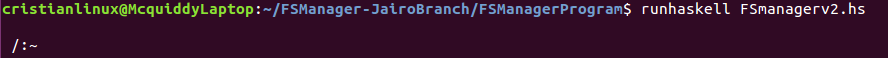
\includegraphics[width=20pc]{run_haskell.png}
\caption{Running the file system.}
\end{figure}

The file system will have all the following components: : 
%Table
\begin{table}

\tbl{REQUIREMENTS}{%
\begin{tabular}{@{}lcp{.30\textwidth}cc@{}}\toprule
HARDWARE& SOFTWARE \\\colrule
1.3 GHz processor& Linux O.S \\
1GHz Ram & Haskell \\
256 MB Video Card & Cabal\\
\botrule
\\\colrule
\end{tabular}}
\end{table}


\begin{itemize}
\item \textbf{Users and Groups.}\newline

%Figure
\begin{figure}[ht]
\centering
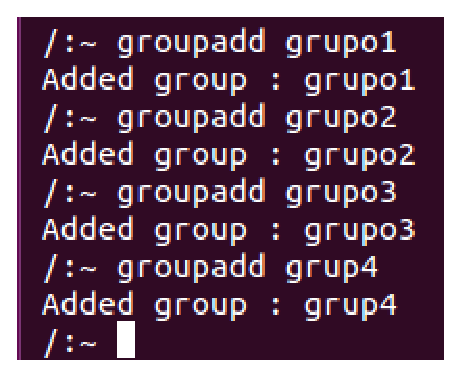
\includegraphics[width=10pc,height=5pc]{addgroups.eps}
\caption{Creating user groups.}
\end{figure}


As figure 4,Groupname, it can be formed by characters (a-z), numbers(0-9) and may only be up to 32 characters long.Group ID (GID),will be a number starting on 1000, It will be automatically added to the groups that are being created in increments of 1.\newline

%Figure
\begin{figure}[ht]
\centering
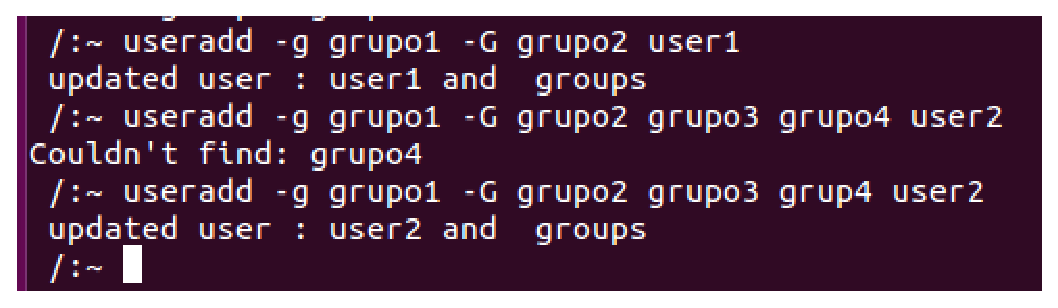
\includegraphics[width=20pc]{addusers.eps}
\caption{Creating users.}
\end{figure}

As figure 5,Username, it can be formed by characters (a-z), numbers(0-9) and may only be up to 32 characters long.

• UserID (UID), this will be a number starting on 1000, It will be automatically added to the users that are being created in increments of 1.

• Home directory, by default it will be set to /home/<username>. When creating a user, this directory has to be automatically created in the system, and the ownership set to the current username and the corresponding primary group.

• Associated primary group. This is a user groups that has to exists in the environment. It will be assigned to the user during the creation with -g , or with the command usermod explained below.

• Associated secondary groups. A user can have multiple groups associated. The group(s) can be assigned to a user during its creation with the -G flag or with the command usermod explained below.

%Figure
\begin{figure}[ht]
\centering
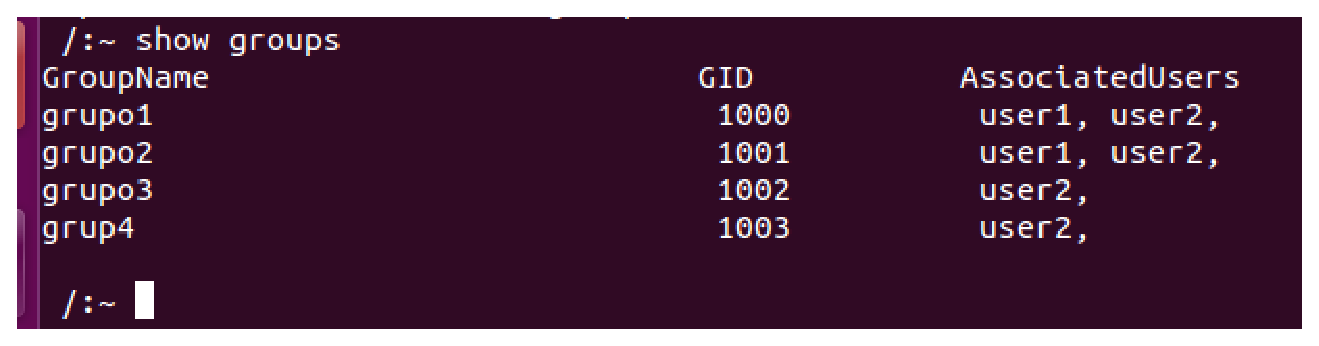
\includegraphics[width=20pc]{showgroups.eps}
\caption{Show groups attributes.}
\end{figure}

The previous command,as figure 6 will be used to list all the existent  groups in the system with their corresponding attributes.

%Figure
\begin{figure}[ht]
\centering
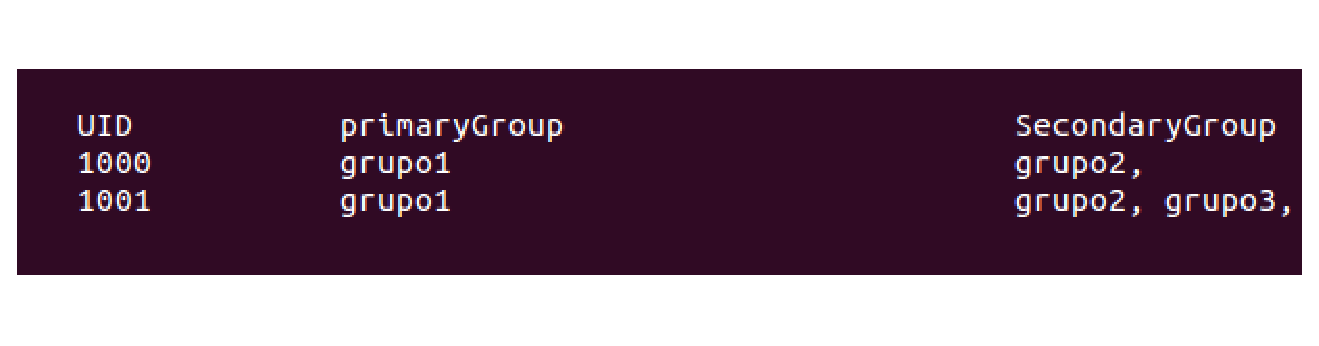
\includegraphics[width=20pc]{showusers.eps}
\caption{Show users attributes.}
\end{figure}


The previous command, as figure 7 will be used to list all the existent user  in the system with their corresponding attributes.
 
 %Figure
\begin{figure}[ht]
\centering
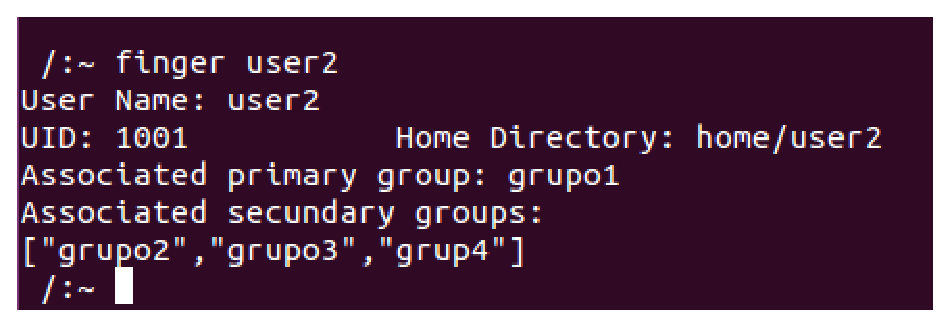
\includegraphics[width=20pc,height=4pc]{fingeruser.eps}
\caption{Finger command.}
\end{figure}

The previous command, as figure 8 ,  show the details of a specific user account.\newline

 %Figure
\begin{figure}[ht]
\centering
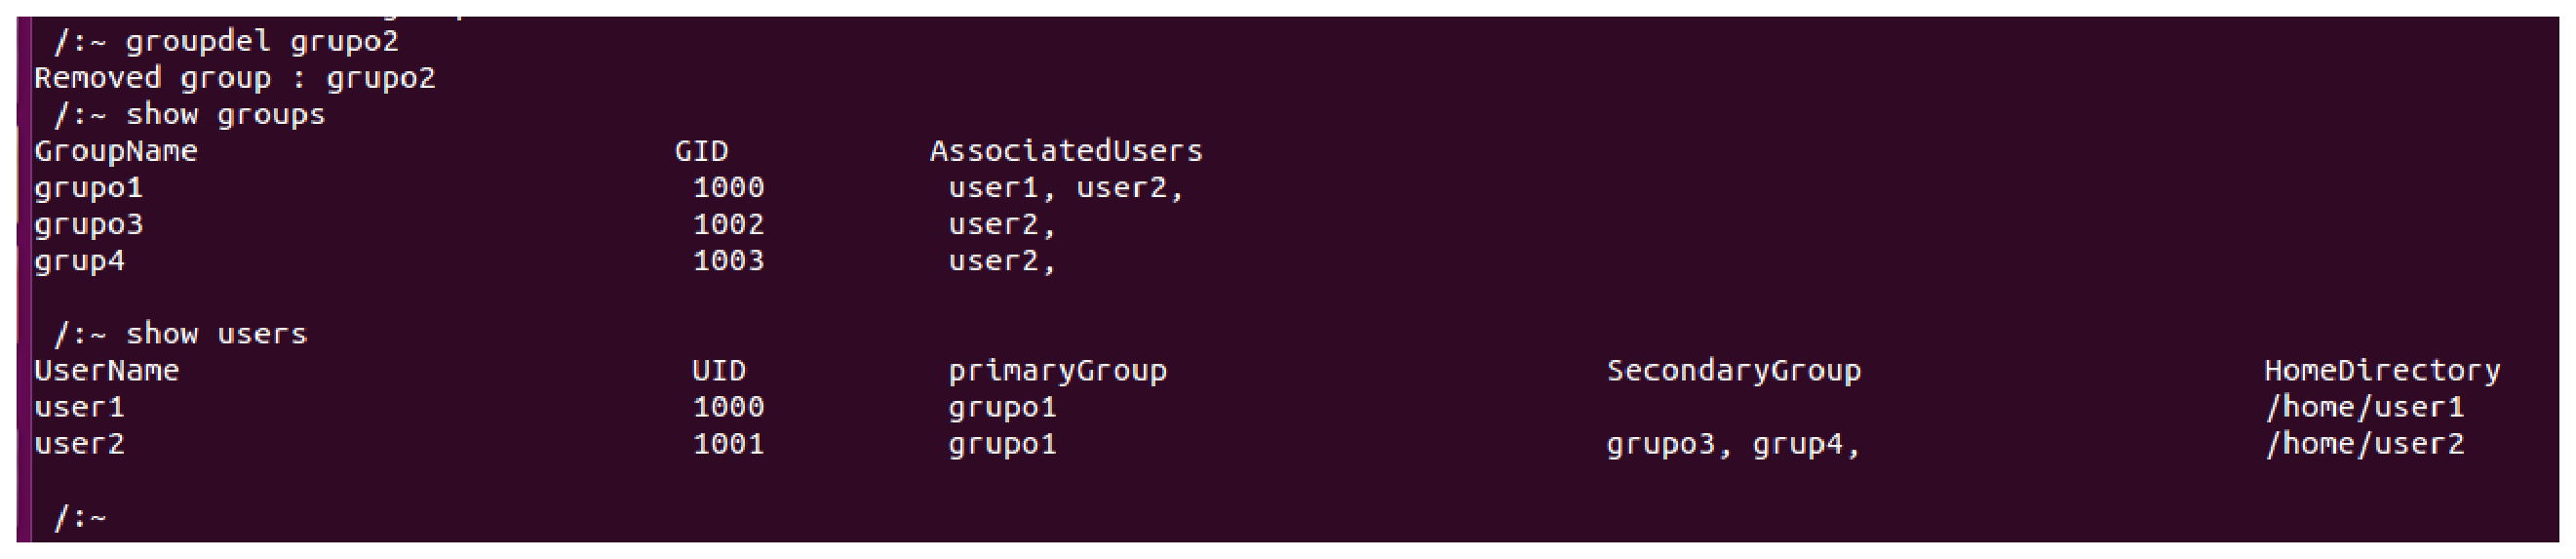
\includegraphics[width=20pc]{delgroup.eps}
\caption{Deleting groups.}
\end{figure}

Groups can be deleted using the previous command, as figure 9. The associated users have to be modified to remove their association with the group that is being removed. Any file or directory with this group in their ownership have to be updated as well to remove from the ownership the group.\newline

 %Figure
\begin{figure}[ht]
\centering
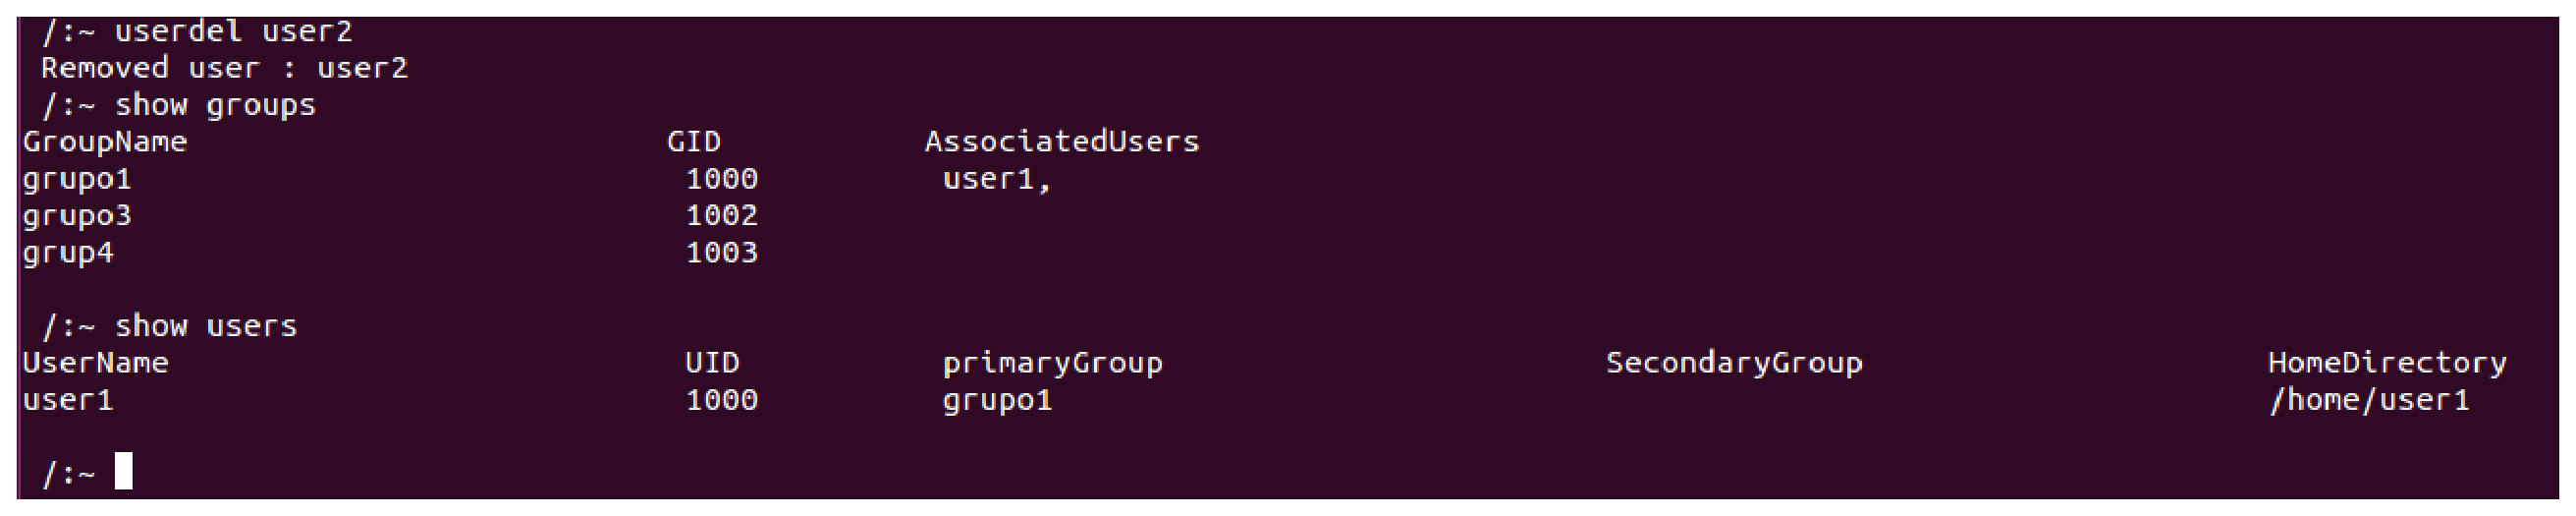
\includegraphics[width=20pc]{deluser.eps}
\caption{Deleting users.}
\end{figure}

Users can be deleted using the previous command, as figure 10. The associated home directory (and any contents) has to be removed when the user is removed as well. Any file or directory with this user in their ownership have to be updated as well to remove from the ownership the username. The groups will have to be updated as well.

%Figure
\begin{figure}[ht]
\centering
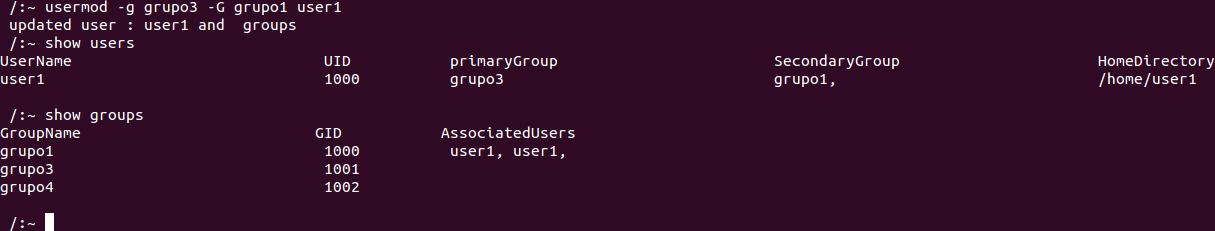
\includegraphics[width=20pc]{usermod.png}
\caption{Modifying users.}
\end{figure}
As figure 11,Users can be modified to change the primary group or to include new secondary groups.\newline

\item \textbf{Storage devices.}\newline
The following command , as figure 12, will create a new storage device.\newline
%Figure
\begin{figure}[ht]
\centering
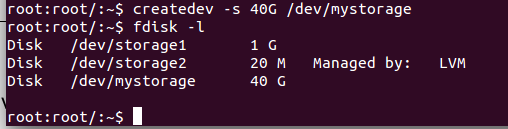
\includegraphics[width=20pc]{storage.png}
\caption{Create storage devices.}
\end{figure}
Storage devices will be created to emulate the equivalent to SAN LUNs, hard drives or any other storage device required to create a file system or a logical volume. \newline
\item \textbf{Volume groups.}\newline
A volume group can be created with the following command, as figure 13. It will be formed by one or more storage devices.
%Figure
\begin{figure}[ht]
\centering
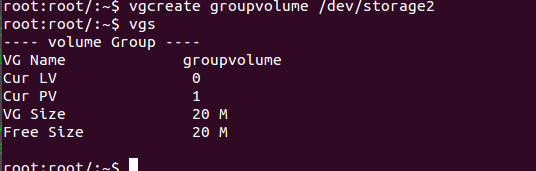
\includegraphics[width=20pc]{volumenes.png}
\caption{Creating volume groupss.}
\end{figure}

 A volume group has the following attributes:\newline
• Volume Group name, it can be formed by characters (a-z), numbers(0-9) and may only be up to 32 characters long.\newline
• List of physical volumes associated. This is the list of storage devices that belong to this volume group.\newline
• Amount of physical volumes associated.\newline
• Amount of volumes created in the volume group.\newline
• List of volumes created in the volume group.\newline
• Total allocated size in MiB. This is the total size of the storage that has been allocated in the volume group. This is a sum of the storage devices sizes that belong to the
specific volume group. \newline
• Total available size in MiB. This is the total space available to be assigned to new or existent volumes.\newline

\item \textbf{Logical volumes.}\newline
A logical volume can be created using the following command, as figure 14. It will be formed by one or more storage devices.
%Figure
\begin{figure}[ht]
\centering

\includegraphics[width=20pc]{logical_volume.png}
\caption{Creating a logical volume.}
\end{figure}
A volume group can have multiple volumes. The size of each volume cannot exceed
the total available space in the volume group at the moment of the volume creation.\newline
\item \textbf{File systems.}\newline
The following command will be used to create a file system and a new directory .
%Figure
\begin{figure}[ht]
\centering
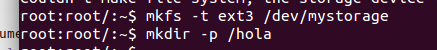
\includegraphics[width=20pc]{file_system.png}
\caption{Creating a file system.}
\end{figure}
The file system type can
be ext2, ext3 or ext4. The size of the file system will be inherit from the logical volume
group or storage device that is being used to create the file system, as figure 15.\newline

\item \textbf{Files and directories.}\newline
All the files and directories will be created over the / (root) directory. This directory (/)
cannot be used as a file system mount point of any newly created file system. It will be
the main parent directory of any directory created in this system.\newline

The below command is going to be used to create directories. Notice the directories can have multiple levels that will be separated with the slash character (/). In the below
example, a mount directory is going to be created and then inside the cristian directory another directory called prueba is going to be created. In order to create file systems of multiple levels use the mkdir command with the -p flag.\newline
 The command \textbf{ cd}  will be used to navigate across all the system directories.\newline

%Figure
\begin{figure}[ht]
\centering
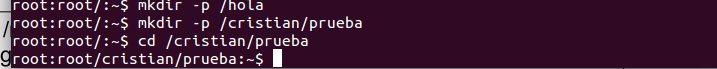
\includegraphics[width=20pc]{directory.png}
\caption{Creating directories and navigating directories.}
\end{figure}
Inside a directory other directories can be created and also files. In order to create a file use the following command: \newline\newline
%Figure
\begin{figure}[ht]
\centering
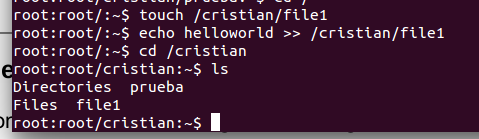
\includegraphics[width=20pc]{files.png}
\caption{Creating empty files and adding contents to a file.}
\end{figure}
Notice the file is created inside the /cristian directory. Other way of creating a file inside a specified directory is being moved inside that directory with the cd command.\newline
Once a file is created we can add contents to such file using \textbf{ echo} ,as figure 17.
\end{itemize}


\section{Project final status}

Symbolic links didn't work \newline

File system mount points didn't work, like mount and unmount.\newline

Remove files didn't works.\newline



\subsection{Some issues or bugs}
\begin{paralist}
\item{}Groupname and userName, it can be formed by characters (a-z), numbers(0-9), symbols and don't have a limit of  characters long\newline
\item{} echo only can write text to a file, without spaces.\newline
\item{}The commands of files system only works without spaces.\newline
\item{}T directories and files are showing unrecursyble

\end{paralist}

\subsection{Challenges during the development}
\begin{paralist}
\item{}Fudgets : Couldn't find module “fudgets”, this  took to make the interface: That was the problem  when trying import the libraty fugets. \newline\newline

Attemps: Download the package fugets and intall with the command cabal install in Fudgets\/hbcr\/hbd\_library and after in Fudgets\/ but did not work.\newline
Write the command cabal update and cabal install but did not work.With the command cabal intall Fudgets, did not work too.\newline
After hours doing the almost the same, it try with other library like, yamba and wxfruit, but doing the same command did not work.
\newline\newline
\item{}Input Text: Design an algorithm that can take the input text.\newline\newline
Solution:   Write the following algorithm :\newline import Control.Monad  \newline     main \= forever \$ do  \newline
putStr "\# " \newline    l $<-$ getLine  \newline   putStrLn  l  \newline\newline 

\item{}Split text :Design a  algorithm that skip the spaces element from the list, when is reading the space element it continue reading the nex element. \newline\newline
Attemps: Write the commands: \newline split( dropBlanks \& oneOf “ “) “ text”, but split one space and not al. \newline The command “dropBlanks, remove all elements of the list that was spliting.\newline
Other command that did not work and not was allowed: splitOn( dropblanks), split(dropBlanks On “”), ect.\newline

Solution: With the command splitOn, make a list with the words without one simbol, in this case is the space “ “, but the problem is when are two or more spaces, because the command split one space, so in the list are spaces like elements.\newline\newline

\item{}Expected IO: When the main call a function this return other type   expected, the error showed was :\newline Couldn't match expected type ‘IO t0’\newline
                with actual type ‘String -> IO ()’\newline
    Probable cause: ‘main’ is applied to too few arguments\newline
    In the expression: main\newline
    When checking the type of the IO action ‘main’\newline

Attemps: 1. Create the main funtion,with arguments, the arguments was sended by the fsManager funtion, who calls the main.\newline
2. Change the name of the main funtion,but the program show de error: Not in scope: ‘main’ Perhaps you meant ‘min’ (imported from Prelude)\newline

Solution: From the main funtion calls the fsManager with the initial arguments, and     from the fsManager gets the input instructions.\newline
\end{paralist}


\section{Conclusions and Suggestions}
Haskell is a strong functional paradigm, but  maintaining code is very inefficient .\newline

Almost everything are connect, so if one function changed the other function need to update.\newline

The modules are very important ans easy to use, they give a better structure of code, when the program are running and show a error message, in the message are the name of the module or file the contain the error, so is faster to fix the problem.\newline

To save or keep the data, this information needs to send from parameter to parameter in each function.\newline

The command x:xs is a good instruction where x take the first element of the list xs, and the function is called recursively, the list xs, is without the first element x.So this, is a faster  and easy way to take the elements of one list.\newline

Casting from IO to String or String to IO, is impossible, the best way is that the function with IO return, take the string and print it.\newline





\begin{thebibliography}{99}


\bibitem{DEK1}
"General Overview Of The Linux File System". Tldp.org. N.p., 2016. Web. 31 May 2016.

\bibitem{DEK2}
Howtogeek.com. (2016). What is the Linux Kernel and What Does It Do?. [online] Available at: http://www.howtogeek.com/howto/31632/what-is-the-linux-kernel-and-what-does-it-do/ [Accessed 8 May 2016].


\bibitem{DEK3}
Prof. Jennifer Vargas , 17 may  2016 , "File System Manager" Costa Rica Institute of Technology.Computer Engineering

\bibitem{DEK4}
Logical Volume Management". Wikipedia. N.p., 2016. Web. 31 May 2016.

\bibitem{DEK5}
2016. [Online]. Available: https://www.sublimetext.com/3. [Accessed: 10- May- 2016].

\bibitem{DEK6}
"Download Haskell Platform". Haskell.org. N.p., 2016. Web. 1 June 2016.

\bibitem{DEK7}
"Chapters - Learn You A Haskell For Great Good!". Learnyouahaskell.com. N.p., 2016. Web. 1 June 2016.

\bibitem{DEK8}
 layout?, How. "How To Understand The Ubuntu File System Layout?". Askubuntu.com. N.p., 2016. Web. 1 June 2016.
 
 \bibitem{DEK9}
 "Logical Volume Management". Wikipedia. N.p., 2016. Web. 1 June 2016.
 
 \bibitem{DEK10}
 "Logical Volume Manager (Linux)". Wikipedia. N.p., 2016. Web. 1 June 2016.
 
 \bibitem{DEK11}
 "Chapter 5. LVM Configuration Examples". Access.redhat.com. N.p., 2016. Web. 1 June 2016.
 
 \bibitem{DEK12}
  "Logical Volume Manager Administration". Access.redhat.com. N.p., 2016. Web. 1 June 2016.
  
 \bibitem{DEK13}
 Perez, Ivan. "On The State Of GUI Programming In Haskell | Keera Studios". Keera.co.uk. N.p., 2014. Web. 1 June 2016.

 \bibitem{DEK14}
"Functional Reactive Programming - Haskellwiki". Wiki.haskell.org. N.p., 2016. Web. 1 June 2016.

 \bibitem{DEK15}
"Haskell Tutorial - Installation". YouTube. N.p., 2016. Web. 1 June 2016.

 \bibitem{DEK16}
"Input And Output - Learn You A Haskell For Great Good!". Learnyouahaskell.com. N.p., 2016. Web. 1 June 2016.

\bibitem{DEK17}
Haskell?, How. "How To Split A String In Haskell?". Stackoverflow.com. N.p., 2016. Web. 1 June 2016.

\bibitem{DEK18}
"How To Work On Lists - Haskellwiki". Wiki.haskell.org. N.p., 2016. Web. 1 June 2016.
\end{thebibliography}

%Table
\begin{table*}[t]
\centering
\tabcolsep8.1pt
\tbl{Details of the activities performed by Cristian Roberto Castillo Mcquiddy}{%
\begin{tabular}{@{}lcp{.60\textwidth}cc@{}}\toprule
Date.& Activity & Description & Hours\\\colrule
 17/05/2016  & Introduccion Haskell      & Research about  what's Haskell, how works the functions, list and tuples. \cite{DEK7} & 2\\
18/05/2016 & Haskell Types & Type variables, type classes ans expresion in haskell. \cite{DEK7} & 2\\
18/05/2016 & Haskell  Recursion & Learning about , A few more recursive functions, algorithm quick sort,Maps and filters,
Lambdas, Function application with \$ \cite{DEK7} & 2\\
19/05/2016 &  How file system works   & Reading the proyect especfications. Learning how fily system in linux works and, like: LVM, logical volumen, physicals volumen. \cite{DEK8} \cite{DEK9} \cite{DEK10} \cite{DEK11}.  & 4\\
 20/05/2016 &  GUI HASKELL Research      & There are GUI libraries IMPERACTIVES likes QT,WX,Gtk+ and FUNTIONAL likes Fudgets and Functional Reactive Programming (FRP) the FUNTIONAL libraries are perfect with this proyect, because it can not use variables . \cite{DEK12} \cite{DEK13} & 1\\
20/05/2016 & Testing Fudgets     &Reading the manual and installing fudgets . \cite{DEK14}.  & 4\\
22/05/2016 & Input Text      & Reading wich command can will use and a algorithm that can take the input text.  \cite{DEK15}& 2\\
22/05/2016& Split text      & Design a  algorithm that skip the spaces element from the list, when is reading the space element it continue reading the nex element. \cite{DEK16} & 4\\
 22/05/2016 & How work a list     & Design algorithm that allowe the estructure of new Group and users \cite{DEK17} & 2\\
23/05/2016 & Groups and users     & Documenting code.The funtion add group and user.  & 1\\
24/05/2016 & How work a list     & Merge the tuples modules   made by  jairo , the program that check the information or data . \cite{DEK18} &3\\
24/05/2016 & Users and Groups    & Creating users and groups & 6\\
25/05/2016 & Users and Groups    & Design an algorithm that update the user and groups list  & 3\\
25/05/2016 & Input Text  and groups  & Remove the spaces of the text an add secondary groups in users& \\ 
25/05/2016 & Symbols input & Detecting and remove some symbols &1\\\botrule
&&Total amount of hours:&40\\\colrule
\end{tabular}}
\end{table*}

%Table
\begin{table*}[t]
\centering


\tabcolsep8.1pt
\tbl{Details of the activities performed by Jairo Méndez Martínez }{%
\begin{tabular}{@{}lcp{.60\textwidth}cc@{}}\toprule
Date.& Activity & Description & Hours\\\colrule
18-05-2016  & Investigation about Haskell   & Research on what is haskell, begins by following a tutorial and initiating its codification. & 3	\\
19-05-2016 & Continue with the investigation about haskell  & Begins the basic approach of the project, raising the structure and requirements for its development and continuing a research on basic functions and functionality haskell lists   & 6 \\
 20-05-2016 &  Investigation about how lists and tuples works in Haskell & continuing research on basic functions and functionality haskell lists, and how to create my own data and my own structure data (a simple linked list) and how to get an element from a list and tuple  & 8\\
21-05-2016 & Inestigation about modules in Haskell   & Finish tha simple linked list, and search how to create a module in haskell and imported from another file   & 3\\
22-0-2016 & Starting to studying and understending the requirements of the proyect  & Generating a table with all the requirements and problems, try & 2\\
 24/05/2016 & Starting to work with groups and users     & Startig to generate the logical of the users and groups, groupadd and useradd & 5\\
 25/05/2016 & Starting with the management of storage devices & Generate the structure of a storage device with a list of tuples, where the information of the device is storage & 4\\
26-05-2016 & Working with volumes  & Implementation of tha functions that will described the functionallity  of them & 15\\
 27-28-29/05/2016 & Working on mkdir and touch functions    & How to generate directories, how to access to them and how to generate files  & 6\\
30-05-2016 & Working with files and directories  & Implementing the logical of the remove, chmod, echo and ls of the files and directories & 11\\
\botrule
&&Total amount of hours:&60\\\colrule
\end{tabular}}

\end{table*}


\end{document}